\section*{Results}

\subsection*{A layered model connects electrical exposure to extracellular particle measurements}

We organized electro-exocytosis as a directed sequence of interacting processes rather than a single exposure--response equation (Fig.~\ref{fig:framework}). Pulse amplitude, width, number, repetition rate, waveform and exposure geometry define the electrical and thermal input. Reduced membrane-charging and permeability states transmit this input to ionic fluxes and organelle responses. Calcium, reactive oxygen species and adenosine triphosphate then regulate remodeling, repair and injury, which in turn determine the balance among small-EV secretion, medium/large-EV budding and apoptotic vesiculation. A separate extracellular and observational layer maps those release pathways to measured particle concentrations and size distributions.

This organization preserves causal interfaces while allowing each layer to be replaced as evidence improves. It also separates two quantities that are commonly conflated: cumulative release from a representative viable producer cell and the particle concentration remaining in sampled medium. The latter depends on viable-cell density, culture volume, extracellular disappearance and the measurement operator. Cargo, potency, purity and manufacturing quantities were retained as downstream outputs but were not fitted to the present particle-size dataset.

\begin{figure}[htbp]
\centering
\includegraphics[width=0.86\textwidth]{figure1_framework.png}
\caption{\textbf{Multiscale organization of the electro-exocytosis model.} The imposed nanosecond pulse is converted to membrane and organelle electrodynamic states, which drive ionic, bioenergetic, remodeling, repair and injury responses. These states regulate multivesicular-body fusion, plasma-membrane budding and injury-associated vesiculation. Released particles enter extracellular kinetic and observation layers before comparison with measured concentration and diameter. Arrows denote modeled causal interfaces rather than experimentally established interactions in a single cell system. ATP, adenosine triphosphate; EV, extracellular vesicle; MVB, multivesicular body; ROS, reactive oxygen species.}
\label{fig:framework}
\end{figure}

\subsection*{Simulations separate reversible, secretion-favored and injury-associated regimes}

Targeted simulations were used to test whether the implemented modules generated internally coherent responses across their different timescales. A mild exposure produced threshold-level membrane charging, limited calcium and oxidative perturbation, substantial resealing and little apoptotic output (Fig.~\ref{fig:regimes}). Increasing electrical forcing increased permeability and calcium loading. When this perturbation was accompanied by effective repair and secretory routing, the model favored small-EV release while retaining viability. When damage exceeded repair capacity, reactive oxygen species accumulated, adenosine triphosphate availability declined and apoptotic-body output increased.

The transition was not determined by electrical dose alone. Calcium buffering reduced phosphatidylserine exposure and remodeling without removing the initial electrodynamic response. Calpain inhibition preferentially reduced actin disruption, whereas stronger annexin- and lysosome-associated repair increased resealing. Within the biogenesis module, limiting Rab/endosomal-sorting activity reduced small-EV release without imposing a uniform reduction on other particle routes; increasing the ceramide-associated secretory bias redirected multivesicular bodies away from lysosomal loss. These comparisons show that similar particle totals can arise from distinct latent mechanisms and can have different viability and purity implications. Individual module trajectories are reported in Supplementary Figs.~1--6.

\begin{figure}[htbp]
\centering
\includegraphics[width=\textwidth]{figure2_regimes.png}
\caption{\textbf{The model distinguishes reversible, secretion-favored and injury-associated response regimes.} Rows show illustrative mild, secretion-favored and injury-associated simulations; columns follow the model from exposure and membrane charging through calcium, oxidative and energetic responses, remodeling and repair, and pathway-resolved particle output. Values are simulated trajectories generated from provisional parameters and are not estimates of biological effect size. Ca$^{2+}$, calcium; EV, extracellular vesicle; ROS, reactive oxygen species.}
\label{fig:regimes}
\end{figure}

\subsection*{Measured particle populations change across diameter and harvest time}

We next examined size-resolved particle measurements from preparations nominally containing $5\times10^6$ CD4$^+$ cells. The supplied dataset contained conditions labelled as one pulse at 20 kV, three pulses at 40 kV and five pulses at 40 kV, sampled 0.5, 1 and 3 h after exposure. Because electrode geometry and delivered field were not available, these labels are treated as source-condition identifiers rather than electric-field amplitudes.

Particles were represented in a common 80--380-nm window using 20-nm bands (Fig.~\ref{fig:sizeprofiles}). Whole-distribution mean diameters remained within approximately 134--147 nm, but individual bands changed nonmonotonically and adjacent diameter ranges sometimes moved in opposite directions between harvests. Total concentration and a single mean-diameter statistic therefore did not capture the observed redistribution. Variability in total concentration within each condition was smaller than variability in distribution shape, which may reflect shared normalization during data export. The independence of repeated measurements and the instrument's detection-limit behavior could not be established from the supplied metadata, so these observations are descriptive rather than inferential.

\begin{figure}[htbp]
\centering
\includegraphics[width=\textwidth]{figure3_size_profiles.png}
\caption{\textbf{Particle-size distributions exhibit condition-dependent temporal redistribution.} Observed concentrations were rebinned into 20-nm bands over 80--380 nm and are shown as mean $\pm$ sample standard deviation; dashed curves show the selected fitted model. Each panel represents one pulse-labelled condition and harvest time. There were three repeated measurements per condition and time except for the three-pulse, 40-kV-labelled condition at 1 h ($n=2$). Repeated-measurement independence was not established, and diameter bands from the same histogram are correlated. Voltage values are unverified source labels, not confirmed delivered fields.}
\label{fig:sizeprofiles}
\end{figure}

\subsection*{A size-resolved observation model captures the dominant distribution but exposes missing dose dependence}

The mechanistic model supplied cumulative per-cell output for three release pathways. We converted release increments to overlapping lognormal size distributions, propagated extracellular particles with a size-dependent first-order loss, and applied an observation matrix over the measured diameter window. Three nested variants were fitted: time-invariant pathway kernels, kernels whose medians responded to matched cell-state trajectories, and state-conditioned kernels with a shared empirical exposure-dependent gain.

The state-conditioned model with the empirical gain achieved the lowest descriptive score. Across nine condition--time targets, the log$_{10}$ root-mean-square error for concentration was 0.1042, equivalent to a typical 1.27-fold difference. The median absolute percentage error was 18.0\%. For normalized size composition, the mean Hellinger distance was 0.0857, the mean Wasserstein distance was 5.00 nm and the mean absolute error in distribution mean diameter was 4.66 nm (Fig.~\ref{fig:calibration}). These are in-sample diagnostics and do not estimate predictive performance.

The time-invariant and state-conditioned kernels produced nearly identical concentration errors before the empirical gain was added (0.1879 log$_{10}$ units for both) and similar Hellinger distances (0.0974 and 0.0973). Thus, changes in kernel median driven by the current upstream trajectories did not explain separation among exposure conditions. The improvement after adding the empirical gain identifies unresolved condition dependence in the upstream model; it does not validate the gain as a biological dose-response mechanism.

The selected fit placed the small-EV and medium/large-EV kernel medians at 121.5 and 201.2 nm, respectively, and estimated an effective extracellular half-life of 0.680 h at 150 nm. The apoptotic-body contribution approached its lower bound. Across 24 optimization starts, 18 endpoints were within 1\% of the best regularized objective. Small- and medium/large-EV medians and the effective half-life were stable across those endpoints, whereas apoptotic-body source conversion varied by more than three orders of magnitude. This parameter is therefore not resolved by the 80--380-nm data. Structured residuals and optimization summaries are shown in Supplementary Figs.~7 and 8.

\begin{figure}[htbp]
\centering
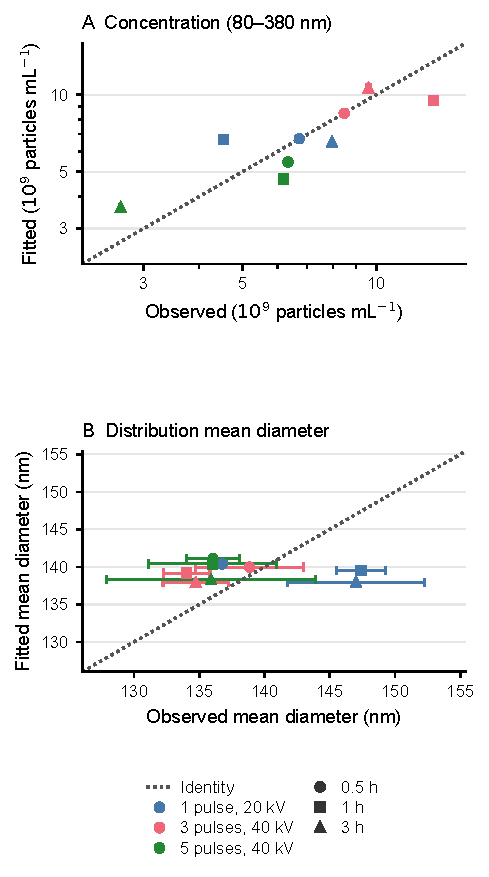
\includegraphics[width=0.72\textwidth]{figure4_calibration.pdf}
\caption{\textbf{The selected observation model reproduces aggregate concentration and mean diameter in sample.} a, Fitted and observed particle concentration integrated over 80--380 nm. b, Fitted and observed whole-histogram mean diameter. Dotted lines indicate identity; horizontal bars show observed sample standard deviations. Colours denote pulse-labelled conditions and symbols denote harvest times. The comparisons use the same observations used for fitting and therefore do not measure out-of-sample prediction.}
\label{fig:calibration}
\end{figure}

\subsection*{Sensitivity separates influential processes from locally constrained parameters}

Morris screening linked simulated extracellular concentration at 3 h primarily to pathway-to-particle source conversion, basal medium/large-EV production and extracellular disappearance (Fig.~\ref{fig:sensitivity}). The largest mean absolute elementary effects in the mechanistic analysis were 0.420 for source conversion, 0.401 for basal medium/large-EV release and 0.401 for the basal budding pool. Effective loss, scission, degradation, uptake and adsorption followed with values between 0.347 and 0.380. The signs of elementary effects agreed with their modeled roles: source and release terms increased concentration, whereas disappearance terms decreased it.

In the observation layer, medium/large- and small-EV source scales had mean absolute elementary effects of 12.98 and 9.34 for the reference condition at 3 h, compared with 2.38 for effective half-life. The empirical gain coefficients were insensitive at the centered reference condition by construction but influential in other conditions. These rankings depend on the provisional ranges and output transformations and should not be interpreted as an experimentally established hierarchy.

Local residual-curvature analysis gave a condition number of $6.3\times10^{21}$, with singular values spanning approximately 22.8 to $2.8\times10^{-10}$. All four apoptotic-body-associated parameters had near-zero local information, consistent with their unstable fitted values. Broad-range sensitivity and local constraint therefore described different properties: a parameter could change the output over a wide range while remaining unconstrained near the selected fit. Conditional Sobol estimates, target-specific sensitivity maps and local-information diagnostics are provided in Supplementary Figs.~9--11.

The combined analysis identified three measurement priorities. Orthogonal particle and pathway-associated measurements are required to separate conversion and recovery from biological release. Additional harvests between 1 and 3 h, accompanied by time-matched sham samples, would distinguish continuing production from extracellular disappearance. Finally, confirmed field dosimetry together with early calcium and injury measurements would test whether the empirical exposure gain can be replaced by an upstream mechanism. The corresponding decision summary is shown in Supplementary Fig.~12.

\begin{figure}[htbp]
\centering
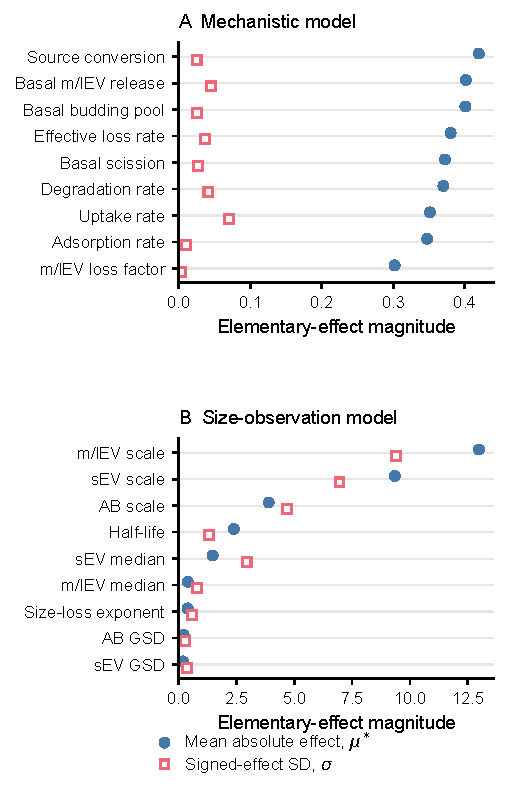
\includegraphics[width=0.78\textwidth]{figure5_sensitivity.pdf}
\caption{\textbf{Parameter influence depends on whether mechanistic or observational output is considered.} a, Morris mean absolute elementary effects for mechanistic extracellular concentration at 3 h. b, Effects for concentration inside the observed 80--380-nm window with upstream trajectories fixed. Circles show mean absolute elementary effects and open squares show the sample standard deviation of signed effects. The mechanistic and observation analyses used different parameter domains and ranges; horizontal magnitudes are therefore not comparable between panels. Two trajectories were used per mechanistic parameter and four per observation parameter. AB, apoptotic body; EV, extracellular vesicle; GSD, geometric standard deviation; m/lEV, medium/large EV; sEV, small EV.}
\label{fig:sensitivity}
\end{figure}
